%!TEX encoding = UTF-8 Unicode
%!TEX root = ../doc-plm.tex


\chapter{Les registres de contrôle}

La déclaration d'un registre de contrôle obéit à une syntaxe particulière, ne serait-ce que parce que son adresse absolue doit y être spécifiée. Pour de nombreux registres, un bit ou un groupe de bits ont une signification particulière, et obtenir la valeur d'un champ ou modifier sa valeur est une opération courante.

À titre d'exemple, nous allons nous intéresser au registre \texttt{ICSR} du processeur ARMv7-M. Le \emph{manuel de référence de l'architecture ARMv7-M}\footnote{\url{http://infocenter.arm.com/help/index.jsp?topic=/com.arm.doc.ddi0403e.b/index.html}} décrit ce registre comme indiqué à la \refFigure{}{definitionICSR}, et indique que son adresse est \texttt{0xE000ED04}.

\begin{figure}[t]
\centering
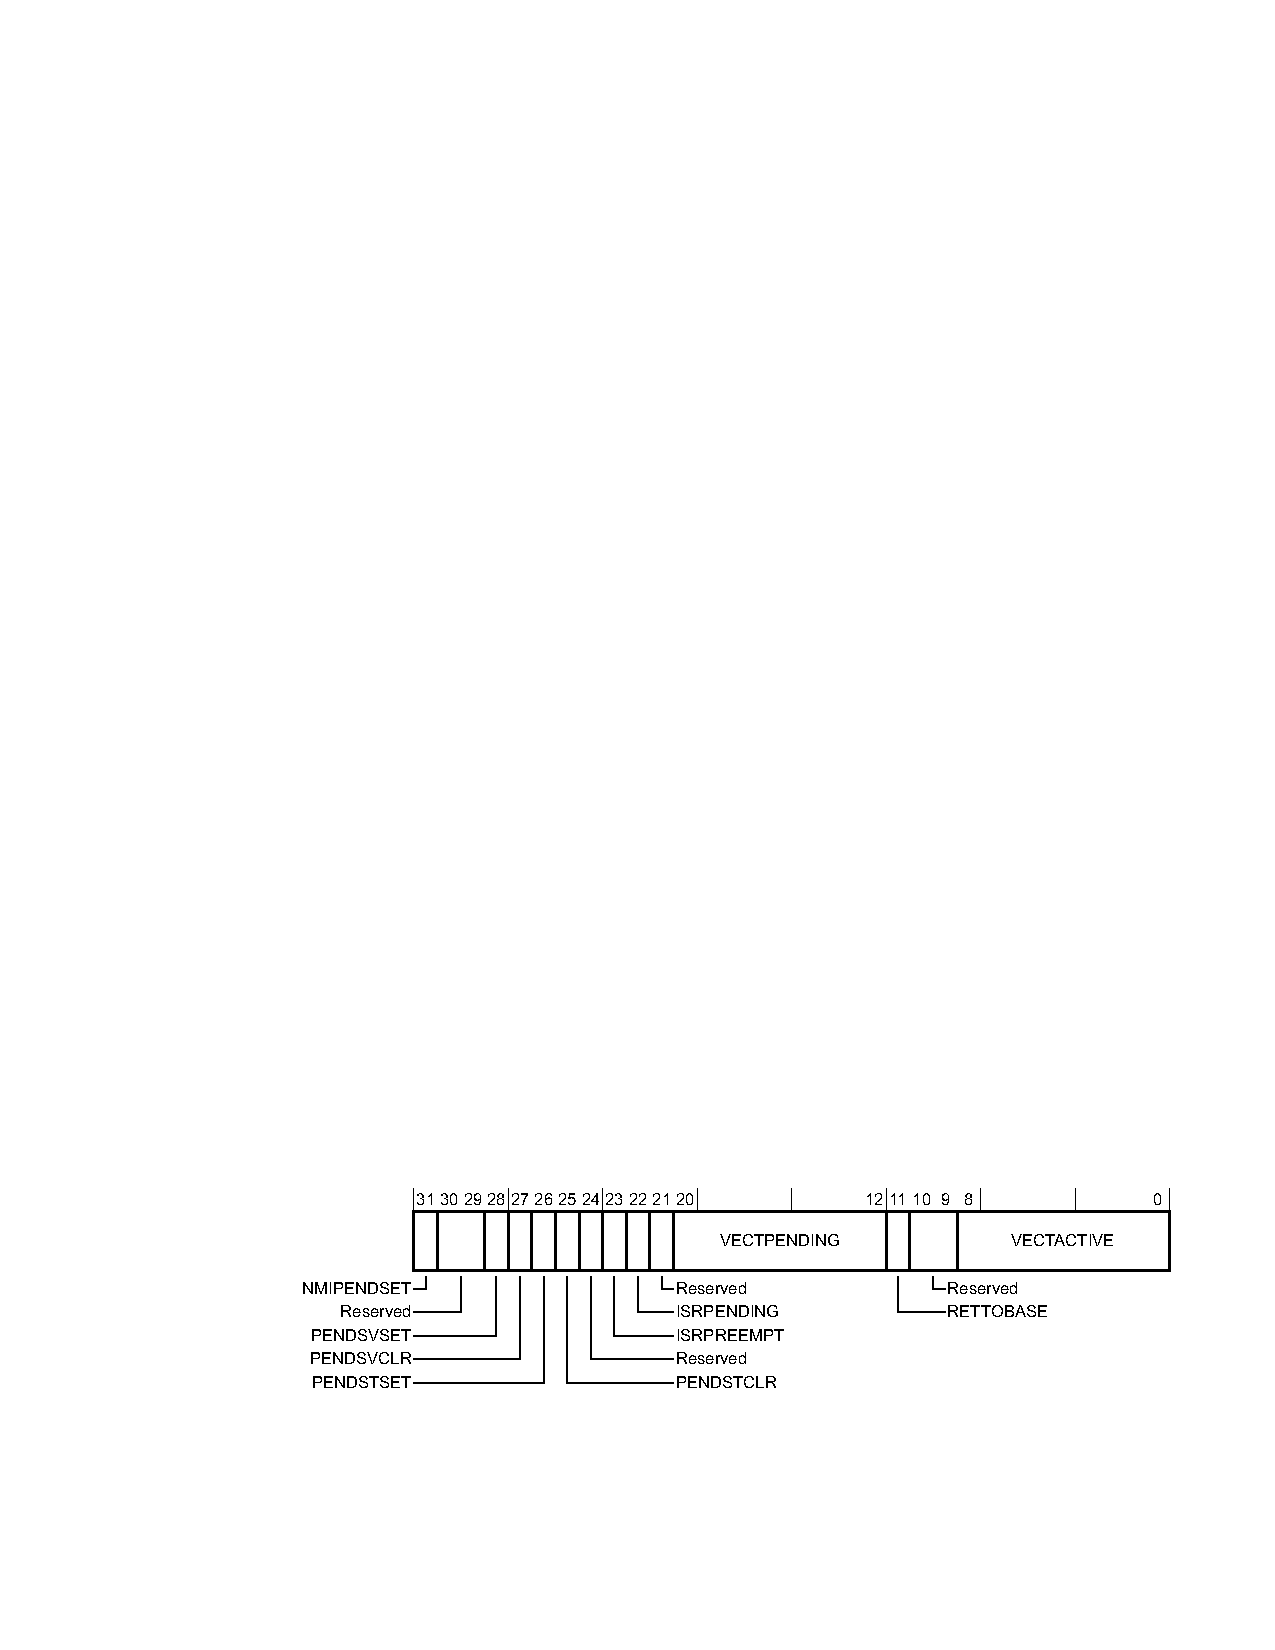
\includegraphics[width=14cm]{chapitres/icsr-armv7m.pdf}
\caption{Registre de contrôle \texttt{ICSR} intégré dans l'ARMv7}
\labelFigure{definitionICSR}
\ligne
\end{figure}




\section{Simple déclaration d'un registre}
Pour déclarer le registre \texttt{ICSR} (\refFigure{}{definitionICSR}), on écrira simplement :
\begin{PLM}
register ICSR at 0xE000_ED04 : UInt32
\end{PLM}

Le type \plm+UInt32+ qui est mentionné signifie que les valeurs écrites et lues de ce registre sont des entiers non signés de 32 bits. Tout type entier, signé ou non signé est autorisé.

Pour lire ou écrire ce registre, on le nomme comme s'il s'agissait d'une simple variable. Par exemple, pour activer l'interruption \texttt{PendSV}, il faut mettre à $1$ le bit \texttt{PENDSVSET}. On écrit donc :
\begin{PLM}
ICSR = 1 << 28
\end{PLM}

Si on voulait activer simultanément les interruptions \texttt{PendSV} et \texttt{SysTick}, il faut mettre à $1$ les bits \texttt{PENDSVSET} et \texttt{PENDSTSET}. On écrit donc :
\begin{PLM}
ICSR = (1 << 28) | (1 << 26)
\end{PLM}

Pour savoir si le bit \texttt{RETTOBASE} est activé, on écrit :
\begin{PLM}
let RETTOBASEActif : Bool = (ICSR & (1 << 11)) != 0
\end{PLM}

Pour accéder à la valeur du champ \texttt{VECTPENDING}, on réalise un masquage :
\begin{PLM}
let vectPending : UInt32 = ICSR & 0x1F_F000
\end{PLM}
 

Et si on veut la valeur de champ justifiée à droite :
\begin{PLM}
let vectPending : UInt32 = (ICSR & 0x1F_F000) >> 12
\end{PLM}
 
Ces écritures peuvent être rendues plus intelligibles en précisant la composition du registre \texttt{ICSR} dans sa déclaration. C'est ce qui va être réalisé dans la section suivante.


\section{Déclaration d'un registre et de ses champs}

%\noindent{\setlength\fboxsep{4pt}\fcolorbox{gray}{green!25!blue!10}{
%\begin{minipage}{0.96\linewidth}
%Peut être qualifiée de\, \index{Temps réel!définition|textbf}\emph{temps réel}\,
% une application informatique qui produit des résultats dont la validité ne dépend pas que de la justesse de leurs valeurs, mais aussi de la date de leur production : un résultat juste ne sera valide que s'il est délivré dans une fenêtre temporelle spécifiée.
%\end{minipage}}}


Lors de la déclaration d'un registre, il est possible de préciser la composition de ses champs entiers et booléens :
\begin{PLM}
register ICSR at 0xE000_ED04 : UInt32 {
  NMIPENDSET, 2, PENDSVSET, PENDSVCLR, PENDSTSET, PENDSTCLR, 1,
  ISRPREEMPT, ISRPENDING, 1, VECTPENDING[9], RETTOBASE, 2, VECTACTIVE[9]
}
\end{PLM}

Entre accolades, trois définitions différentes peuvent apparaître :
\begin{itemize}
\item un nombre indique le nombre de bits consécutifs inutilisés ;
\item un identificateur (par exemple \texttt{NMIPENDSET}) nomme un champ booléen ;
\item un identificateur suivi d'un nombre entre crochets (par exemple \texttt{VECTPENDING[9]}) nomme un champ entier constitué du nombre indiqué de bits consécutifs.
\end{itemize}

La description commence par le bit le plus significatif : comme le type du registre est \plm+UInt32+ (entier non signé sur 32 bits), le premier bit nommé \texttt{NMIPENDSET} porte le n°31, \texttt{PENDSVSET} le n°28, ...

Cette écriture n'est autorisée que si le type nommé (ici \plm+UInt32+) est une type entier non signé. Les types signés (\plm+Int32+, ...) sont interdits. Le compilateur vérifie que la description des champs définit exactement le nombre de bits du type nommé, ici les 32 bits du type \plm+UInt32+.










\subsection{Accès en lecture aux champs booléens}
Pour accéder à la valeur d'un champ, on utilise la notation pointée en nommant ce champ :
\begin{PLM}
let x : UInt32 = ICSR.ISRPENDING // 0 ou 2**22
\end{PLM}
Ceci effectue simplement un masquage de façon à isoler le bit demandé. Aucun décalage n'est réalisé. Comme le bit \texttt{ISRPENDING} est le 22\up{e}, le résultat est $0$ ou $2^{22}$.

Si l'on veut obtenir un résultat justifié à droite, on utilise en plus l'accesseur \plm+.shift+ :
\begin{PLM}
let x : UInt32 = ICSR.ISRPENDING.shift // 0 ou 1
\end{PLM}

L'accesseur  \plm+.bool+ permet d'obtenir une valeur booléenne correspondant à la valeur d'un bit d'un registre :
\begin{PLM}
let x : Bool = ICSR.ISRPENDING.bool // false ou true
\end{PLM}











\subsection{Accès en lecture aux champs entiers}

Comme pour un champ booléen, l'accès à un champ entier s'effectue par la notation pointée \plm+.+. Par exemple :
\begin{PLM}
let x : UInt32 = ICSR.VECTPENDING // (0 a 2**9-1) << 12
\end{PLM}

\plm+ICSR.VECTPENDING+ applique un masquage de la valeur de \plm+ICSR+ pour ne conserver que les bits correspondants au champ \plm+VECTPENDING+. Aucun décalage n'est effectué.


Pour obtenir une valeur justifiée à droite, on ajoute l'accesseur \plm+.shift+ :
\begin{PLM}
let x : UInt32 = ICSR.VECTPENDING.shift // Entre 0 et 2**9-1
\end{PLM}

La valeur renvoyée est alors comprise en $0$ et $2^9-1$.



\subsection{Constantes associées aux champs booléens}

Le délimiteur \plm+::+ permet de définir des constantes correspondant aux bits d'un registre. Par exemple, pour activer l'interruption \texttt{PendSV}, il faut mettre à $1$ le bit \texttt{PENDSVSET}. On écrit donc :
\begin{PLM}
ICSR = ICSR::PENDSVSET
\end{PLM}

La constante \plm+ICSR::PENDSVSET+ a le type du registre \plm+ICSR+, c'est-à-dire \plm+UInt32+.

De façon analogue, si on voulait activer simultanément les interruptions \texttt{PendSV} et \texttt{SysTick}, il faut mettre à $1$ les bits \texttt{PENDSVSET} et \texttt{PENDSTSET}. On écrit donc :
\begin{PLM}
ICSR = ICSR::PENDSVSET | ICSR::PENDSTSET
\end{PLM}






\subsectionLabel{Expressions associées aux champs entiers}{constructionChampEntierRegistre}

Le délimiteur \plm+::+ permet de simplifier la composition d'une valeur correspondant à un champ entier. Par exemple :

\begin{PLM}
let y : UInt32 = ICSR::VECTPENDING (x) // x : expression entière non signée
\end{PLM}

Le champ \texttt{VECTPENDING} est un champ de 9 bits, il peut donc accepter une valeur entière entre $0$ et $511$. L'expression \plm+x+ doit être de type entier non signé. Plusieurs cas sont à considérer :
\begin{itemize}
\item si \plm+x+ est une expression statique, alors le compilateur vérifie que sa valeur est comprise entre $0$ et $511$ (un message d'erreur de compilation est émis dans le cas contraire) ; l'expression \plm+ICSR::VECTPENDING (x)+ est alors aussi une expression statique ;
\item si \plm+x+ est une expression non calculable statiquement :
  \begin{itemize}
  \item si \plm+x+ est du type \plm+UInt8+, alors toute valeur de \plm+x+ est acceptable : le code engendré se borne à faire le décalage à gauche de la valeur de \plm+x+ ;
  \item sinon, une assertion (code : voir \refTableauPage{tableauCodeExceptions}) est engendrée ; la valeur de \plm+x+ est ensuite masquée pour pallier un éventuel débordement, puis décalée. 
  \end{itemize}
\end{itemize}

D'une manière générale, si \plm+x+ n'est pas calculable statiquement, le code engendré ne comprendra pas d'assertion si le nombre de bits du champ est supérieur ou égal au nombre de bits du type entier de l'expression.





\subsection{Masques associés aux champs entiers}

Le délimiteur \plm+::+ permet de simplifier la composition d'un masque correspondant à un champ entier. Par exemple :

\begin{PLM}
let y : UInt32 = ICSR::VECTPENDING // y vaut 0x1F_F000
\end{PLM}

Le champ \texttt{VECTPENDING} est un champ de 9 bits commençant au bit 12. La valeur du masque \plm+ICSR::VECTPENDING+ est donc $(2^9 - 1)^{12}$, soit \texttt{0x1F\_F000}.

Les masques ainsi obtenus sont des expressions statiques.









\section{Attribut \texttt{@ro}}
La déclaration d'un registre accepte l'attribut \plm+@ro+, qui signifie qu'il est en lecture seule. Par exemple :
\begin{PLM}
register SYST_CALIB @ro at 0xE000_E01C : UInt32
\end{PLM}

Toute tentative de faire figurer ce registre dans une construction qui provoque une écriture de celui-ci entraîne l'apparition d'une erreur de compilation.


\section{Déclaration de plusieurs registres}

Il est possible de regrouper les déclarations de registres partageant la même décomposition de leur champs. Par exemple, pour les registres \texttt{PORT$n$\_PCR$m$} du \texttt{mk20dx256} (seule la déclaration de deux registres est montrée) :

\begin{PLM}
register
  PORTA_PCR0 at 0x4004_9000
  PORTA_PCR1 at 0x4004_9004
: UInt32 {
  7, isf, 4, irqc[4], lk, 4, mux[3], 1, dse, ode, pfe, 1, sre, pe, ps
}
\end{PLM}

